%!TEX root = ../../Master.tex
\section{Graph theory}

Graph theory is frequently used in computer science to model some kind of relationship between objects. These objects could be anything. Graph theory is a preferred method to model building complexes, because it can precisely model how e.g. a hallway in a hospital is connected to a room.

In graph theory objects are called \enquote{nodes} or \enquote{vertices}. The two terms can be used interchangeably. In this paper, vertices will describe coordinates or POI (points of interest) in a hospital. Another term in graph theory is an edge. This is basically connecting two vertices and thereby providing a relationship between these vertices. See \cref{fig:labeled_graph}. An edge can be seen as a possible route connecting one coordinate to another. Now in order to describe the relationship between two vertices, we use an weighted graph in which an edge has a number attribute called a weight. A weight can describe the time, distance or any other metric that in some way can describe how two connected vertices are related.\cite{wiki_graph_glos,MIT2012}

We can describe these definitions formally.\cite{MIT2012}
\begin{mydef}
	A graph $G$ is a pair of sets $(V,E)$ where $V$ is a non-empty set of items called vertices or nodes. $E$ is a set of 2-item subsets of $V$ called edges.
\end{mydef}

\begin{figure}[ht!]
    \centering
    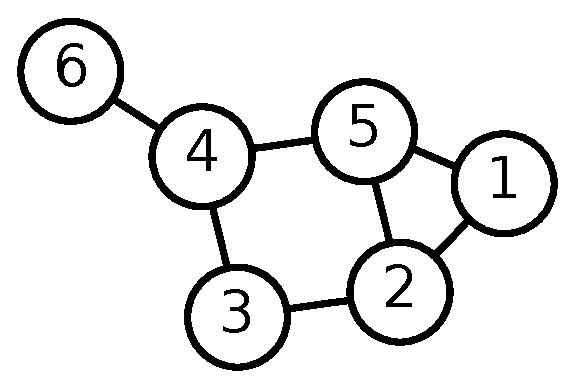
\includegraphics[width=0.5\textwidth]{6n-graf.eps}
    \caption{A labeled simple graph with vertex set $V = \left\{ {1, 2, 3, 4, 5, 6} \right\} $ and edge set $E = \left\{ \left\{ {1,2}\right\}, \left\{ {1,5}\right\}, \left\{ {2,3}\right\}, \left\{ {2,5}\right\}, \left\{ {3,4}\right\}, \left\{ {4,5} \right\} , \left\{ {4,6} \right\} \right\}$. \cite{wiki_graph_glos}}
    \label{fig:labeled_graph}
  \end{figure}

\subsection{Storing a complex as a graph}

\subsubsection{Representing a floor}

Every decision and every change direct is a vertex in our graph, is modelled by vertices connected with edges. Exits, elevators, stair and bridges are vertices for getting from a floor to another, including another building. Vertices that does not classify as one of the previously mentioned are doors, intersection and a change of walking direction. Connecting the vertices are edges with a weight, which could be weighted with the distance in meters from one vertex to another.

\begin{figure}[ht!]
    \centering
    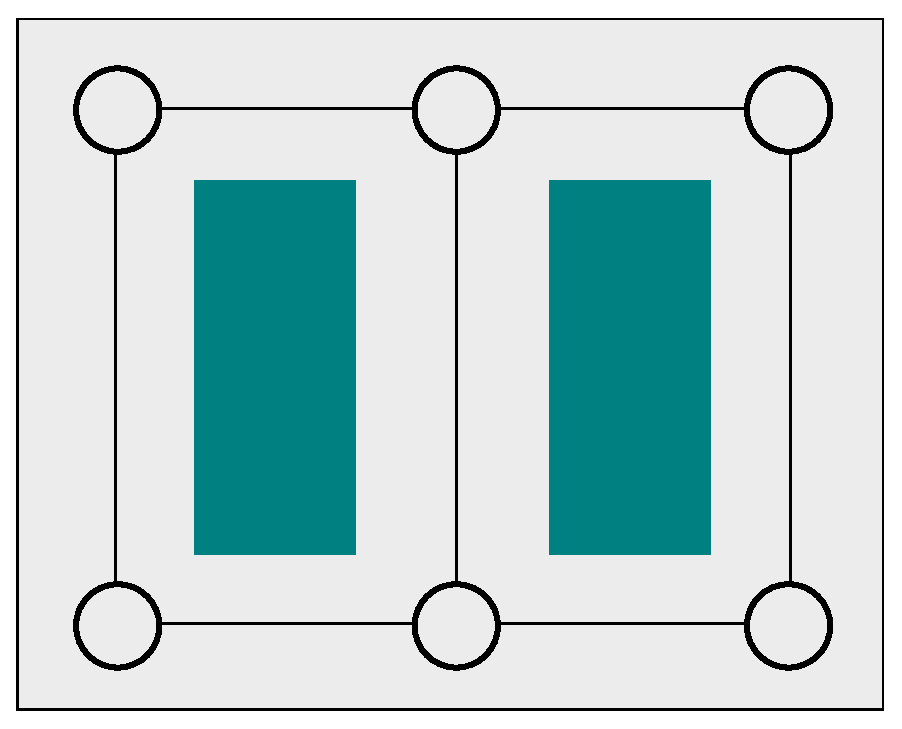
\includegraphics[width=0.5\textwidth]{Vertices}
    \caption{Representation of detail in modelling a floor}
    \label{fig:Vertices}
  \end{figure}

\subsubsection{Multiple floors}

A complex such as a hospital usually consist of multiple floors, connected by stairs and elevators as observed at the visit to Sygehus Nord. Representing floors in a graph could be shown by having edges in between different floors. Elevators or stairs represented by vertices that connects the edges between the floors. Having a graph that models the whole complex can have complications such as overlapping vertices coordinates. Estimating a heuristic value between destination and vertices on the other side of, such as floors. Means that the heuristic models that does not account for obstacles, would cause the A* algorithm to expand vertices, leading to vertices below the destination on a separate floor than the desired.

\begin{figure}[ht!]
    \centering
    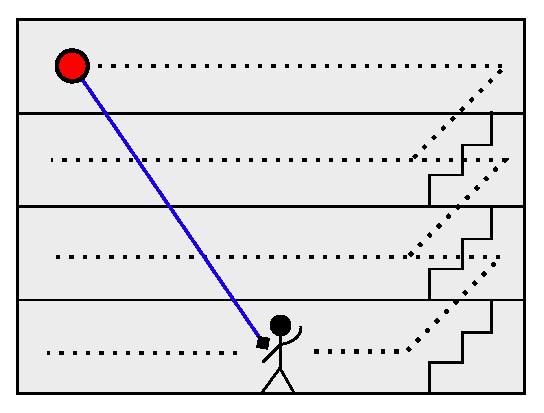
\includegraphics[width=0.5\textwidth]{buildingAstar}
    \caption{How many vertices the A* algorithm would expand, if using the euclidean distance as heuristic}
    \label{fig:buildingAstar}
  \end{figure}

If the complex is divided into separate floor graphs, the algorithm would not have to account for the z coordinate in its heuristic value. A algorithm could evaluate if the source and destination is on the same floor, if not the algorithm could divide the problem into A* searches. First finding a path leading to an elevator or stair which lead the destinations floor. The optimal path from one floor to another can be pre-calculated and stored. 

\begin{figure}[ht!]
    \centering
    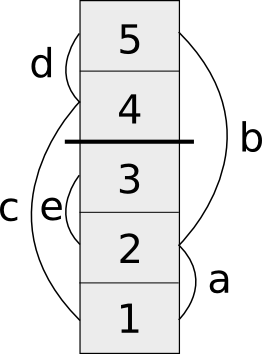
\includegraphics[width=0.5\textwidth]{PekhoeS}
    \caption{Visual representation of floors}
    \label{fig:PekhoeS}
  \end{figure}

\subsubsection{Multiple buildings}

The previously described method for modelling floors allows the algorithm to comprehend from complexes of multiple buildings. By not having to account for a complex with multiple buildings and floors, each floor would have its own identification. Allowing for an exit from one building to another through a bridge. This simplifies a lookup if an individual is the destination floor height physically but not in the right building, because a floor height is not relevant.
